\chapter{Ajout du support CAN}
{Objectifs:
  \begin{itemize}
  \item Ajouter de nouveaux paquets à compiler
  \item Configurer un périphérique hardware (CAN) sous la RPi3
  \item Tester le nouveau système
  \end{itemize}
}

\section{Avant de commencer...}

Le controlleur CAN que nous allons utiliser est un
\href{https://www.microchip.com/wwwproducts/en/en010406}{MCP2515} qui utilise
un bus SPI.

Prendre un peu de temps pour lire la datasheet du MCP2515, regarder les
différentes pins, le voltage en entrée, etc. Cela vous permettra de comprendre
les pins suivantes utilisées.

Nous allons utiliser les pins SPI de la RPi : \\

\begin{centering}
  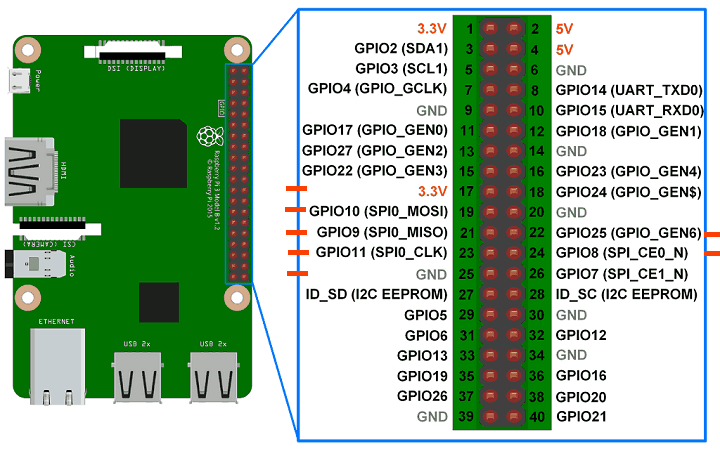
\includegraphics[height=0.3\textheight]{pictures/04_labs/rpi3_gpio_layout_spi.png} \\
\end{centering}

Ce qui nous donnera une connexion SPI suivante : \\

\begin{centering}
  \includegraphics[height=0.3\textheight]{graphics/04_labs/rpi3_mcp2515.pdf} \\
\end{centering}

\section{Configuration}
\subsection{Configuration de la RPi3 : defconfig + device-tree}

Pour ajouter le support d'un périphérique dans Linux, il faut:
\begin{itemize}
\item Ajouter un noeud dans le device tree selon le bus utilisé
\item Activer le driver dans la configuration kernel
\end{itemize}

\subsubsection{Device-tree overlay}

La RPi a une particularité par rapport à certaines cartes de développpement,
elle utilise un fichier de configuration de type texte pour faire des
modifications hardware via un firmware.

Rechercher ce fichier :

\begin{verbatim}
$ find . -iname config.txt
./package/rpi-firmware/config.txt
\end{verbatim}

Lire les fichiers contenus dans le dossier \code{board/raspberrypi3/}.

Regarder comment est-il possible de modifier le fichier \code{config.txt},
notamment avec ce qui est déjà effectué avec l'option \code{dtoverlay=pi3-miniuart-bt}.
Les informations sur la syntaxe de ce fichier sont disponibles sur ce site
\url{http://elinux.org/RPiconfig}. Les dtoverlay permettent d'activer des
parties hardware de la raspberry pi en modifiant le Device Tree.

Pour activer le bus SPI, il faut utiliser le \code{dtparam} et pour activer le
hardware CS, ça sera via \code{dtoverlay} (voir la documentation \href{https://github.com/raspberrypi/firmware/blob/master/boot/overlays/README#L2103..L2106}{ici}):
\begin{verbatim}
dtparam=spi=on
dtoverlay=spi0-hw-cs
\end{verbatim}

En ce qui concerne le chip CAN, il faut utiliser un \code{dtoverlay}.
Voici une \href{https://github.com/raspberrypi/firmware/blob/master/boot/overlays/README#L56}{documentation}
à lire concernant leur utilisation avec la node du controlleur CAN que nous
utiliserons \href{https://github.com/raspberrypi/firmware/blob/master/boot/overlays/README#L1478..L1485}{MCP2515}.
\begin{verbatim}
dtoverlay=mcp2515-can0,oscillator=16000000,interrupt=25
\end{verbatim}

Toutes ces nouvelles valeurs devront être ajoutées dans le fichier \code{config.txt}
en ajoutant du code dans le script \code{post-image.sh} de la RPi3. Prendre
exemple sur les autres arguments pour ajouter une option \code{--add-mcp2515-overlay}.

Une fois que le script a été modifié, il faudra ajouter l'option dans la
configuration Buildroot (cf variable \code{BR2_ROOTFS_POST_SCRIPT_ARGS}).

\begin{centering}
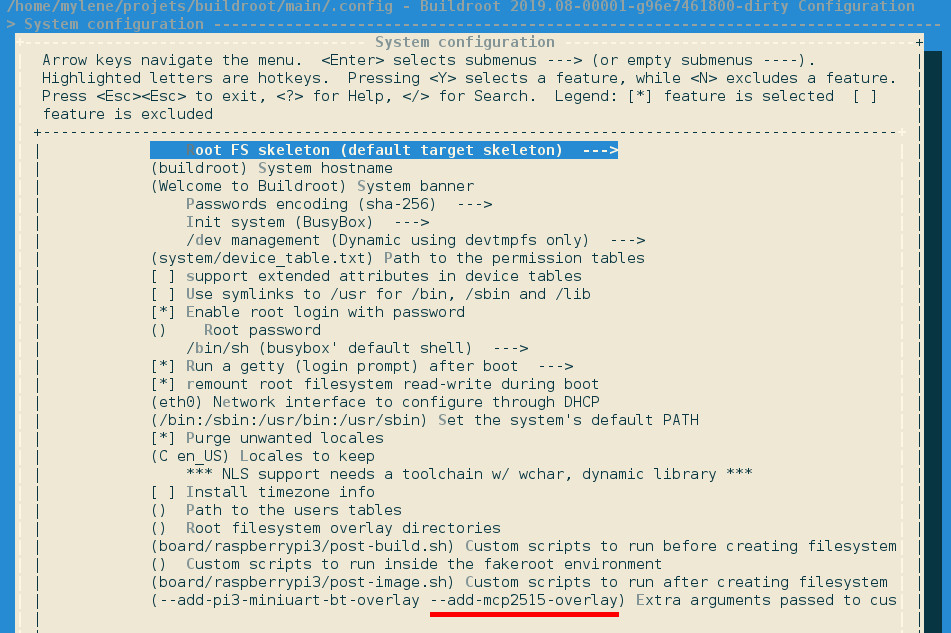
\includegraphics[height=0.3\textheight]{pictures/04_labs/config_br_overlay.jpg} \\
\end{centering}

\subsubsection{Configuration kernel}

Par défaut, le driver pour le controlleur CAN MCP2515 est déjà activé dans
la configuration que l'on utilise du kernel.

Vérifier que la configuration \code{MCP251X} est activée (soit builtin \code{=y}
soit en module \code{=m}) en utilisant la commande suivante :

\begin{verbatim}
make linux-menuconfig
\end{verbatim}

Cela vous ouvrira le menuconfig spécifique au kernel (et non pas à Buildroot).

\subsection{Configuration de Buildroot}

Maintenant que la configuration coté Kernel et device-tree est réalisée, il
faut activer des nouveaux paquets dans Buildroot pour pouvoir avoir des
outils pour utiliser le CAN :
\begin{itemize}
\item \texttt{LIBSOCKETCAN} : Permet de controller un périphérique CAN via du code en C
\item \texttt{CAN\_UTILS} : Permet d'ajouter des outils en ligne de commande pour
  tester des périphériques CAN tel que \code{candump} et \code{cansend}.
\end{itemize}

Ouvrir le menuconfig de buildroot et chercher les paquets qui nous intéressent.
Les activer, sauvegarder votre configuration et compiler une nouvelle image.

\subsection{Compilation et test}

Vérifier qu'ils sont bien compilés pour votre RPi3 avec :

\begin{verbatim}
$ find output/target/ -iname can*
\end{verbatim}

\begin{centering}
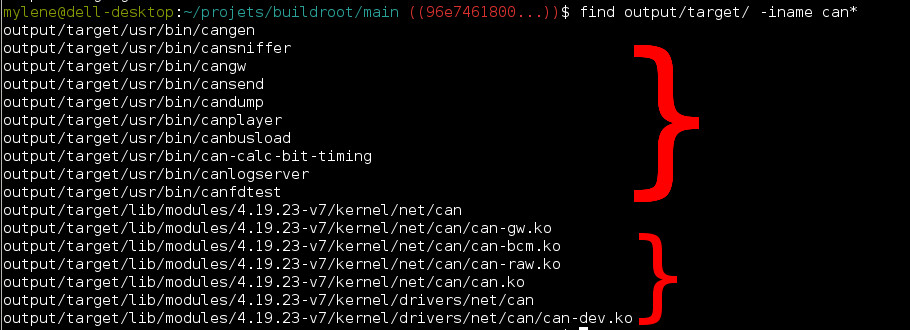
\includegraphics[height=0.2\textheight]{pictures/04_labs/output_target.jpg} \\
\end{centering}

\begin{verbatim}
$ find output/staging/ -iname can*
\end{verbatim}

\begin{centering}
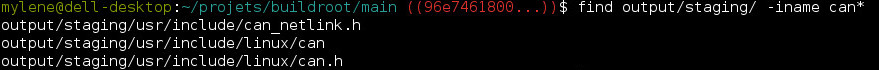
\includegraphics[height=0.05\textheight]{pictures/04_labs/output_staging.jpg} \\
\end{centering}

Maintenant, flasher votre carte SD avec votre nouvelle image, booter votre
RPi3 avec le module CAN connecté comme il faut et tester votre interface
\code{can0} avec :

\begin{verbatim}
$ ip link set can0 up type can bitrate 500000
$ ifconfig
$ cansend can0 01a#11223344AABBCCDD
$ candump can0
\end{verbatim}

\subsection{Un peu d'overlay}

Pour activer automatiquement l'interface CAN au boot, on va utiliser
une règle UDEV. Pour cela, on utilisera le système d'overlay dans Buildroot.

Lire la documentation de Buildroot sur les
\href{https://buildroot.org/downloads/manual/manual.html#rootfs-custom}{overlays}
et notamment la variable \texttt{BR2\_ROOTFS\_OVERLAY},
la documentation sur les
\href{https://www.linuxembedded.fr/2015/05/une-introduction-a-udev/}{règles udev}.

Créer un overlay pour la RPi3 pour créer une règle UDEV \code{can.rules}
suivante :

\begin{verbatim}
SUBSYSTEM=="net", DEVPATH=="/devices/platform/soc/3f204000.spi/spi_master/spi0/spi0.0/net/can0", \
RUN+="/sbin/ip link set can0 up type can bitrate 500000"
\end{verbatim}

Configurer Buildroot pour prendre en compte votre overlay. Vérifier que votre
règle est bien installée dans le dossier \code{target} :

\begin{verbatim}
$ find . -iname can.rules
./board/raspberrypi/overlay/etc/udev/rules.d/can.rules
./output/target/etc/udev/rules.d/can.rules
\end{verbatim}

Et, une fois le rootfs installé sur votre carte SD, que l'interface CAN
est automatiquement montée :
\begin{verbatim}
$ ifconfig
\end{verbatim}
